\documentclass[a4paper]{article}
\usepackage[utf8]{inputenc}
\usepackage[portuguese]{babel}
\usepackage{a4wide}
\usepackage{graphicx}
\usepackage{float}
\usepackage{scrextend}
\usepackage[normalem]{ulem}
\usepackage{indentfirst}
\useunder{\uline}{\ul}{}

\title{Projeto de Laboratórios de Informática 1\\Grupo LI1g057}
\author{Rui Azevedo (A80789) \and Daniel Costa (A81302)}
\date{\today}

\begin{document}

\maketitle

\begin{figure}[H]
      \centering
      
\includegraphics[width=8cm]{UMINHO.jpg}
\end{figure}

\newpage

\begin{abstract}
\label{sec:Resumo}
Este trabalho, desenvolvido no âmbito da disciplina de \emph{Laboratórios de Informática}, tem como objetivo o desenvolvimento do jogo Bomberman usando a linguagem funcional \emph{Haskell}.\par O trabalho foi desenvolvido em seis tarefas distintas: implementação do mapa, movimento dos jogadores, compressão e descompressão do jogo, passagem do tempo, criação do ambiente gráfico usando \emph{Gloss} e por último a implementação da estratégia de jogo. \par Neste relatório iremos fazer uma pequena descrição de cada tarefa individualmente, assim como a nossa abordagem ao problema em questão apresentando alguns exemplos de código. As diferentes tarefas foram desenvolvidas segundo um enunciado que foi fornecido pelos docentes da Unidade Curricular a fim de nos guiar no desenvolvimento do trabalho.
\end{abstract}

\vspace{1cm}

\tableofcontents

\vspace{1cm}

\section{Introdução}
\label{sec:Intro}
O trabalho desenvolvido foi repartido por seis tarefas, onde cada uma tinha um enunciado com o objetivo da mesma e alguns pontos importantes em termos em atenção assim como alguns exemplos. O código de cada tarefa foi submetido e avaliado na plataforma \emph{SVN} onde, uma vez submetida uma tarefa sabíamos se esta estava a passar aos testes impostos pelos docentes.\par A nossa abordagem ao problema vai de encontro ao pedido no enunciado de cada tarefa e, após uma reflexão lógica do problema e de um estruturamento de ideias, demos seguimento ao início de cada tarefa. Neste relatório vamos descrever os problemas em causa assim como os objetivos que pretendemos alcançar, resumindo o problema de cada tarefa. 

\newpage

\section{Descrição do problema}
O objetivo do trabalho é a implementação do jogo \emph{Bomberman} na linguagem funcional \emph{Haskell}.\par O trabalho é composto por seis tarefas, cada uma com um objetivo. Inicialmente, o propósito foi criar o mapa do jogo (dimensão $n$, sendo $n$ um número ímpar maior ou igual a 5) onde o contorno do mapa é composto por pedras assim como cada linha ou coluna, alternadamente, (cada pedra é representada por um '\#'), e cada célula pode ser vazia, conter um bloco de pedra indestrutível ou um bloco de tijolo destrutível por uma bomba. Alguns blocos de tijolo podem esconder um power-up (Bombs ou Flames), que servem para aumentar a capacidade de um jogador. Os jogadores podem lançar bombas, cujo tempo de detonação são 10 segundos e cujo raio de impacto varia, e estas podem matar outros jogadores ou influenciar o tempo de detonação de uma outra bomba lançada por outro jogador (dependendo do raio de impacto da bomba). Os possíveis movimentos de um jogador são: cima (U), baixo (D), direita (R) ou esquerda (L).  

\vspace{0.5cm}
\section{Concepção da Solução}
\label{sec:solucao}

\subsection{Tarefa 1} O objetivo desta tarefa é fazer a implementação do mapa do jogo. Como foi referido anteriormente, o mapa do jogo é composto por pedras no seu contorno, em cada linha ou coluna, alternadamente, e cada célula pode ser vazia, conter um bloco de pedra indestrutível ou um bloco de tijolo destrutível por uma bomba. Os quatro cantos do mapa têm sempre três espaços vazios para os jogadores puderem dar início ao jogo. Nós decidimos fazer exemplos de mapa em \emph{Excel} a fim de estruturar o nosso raciocínio. De seguida, apresentamos um desses exemplos:

\noindent
\begin{figure}[!htb]
      \centering
      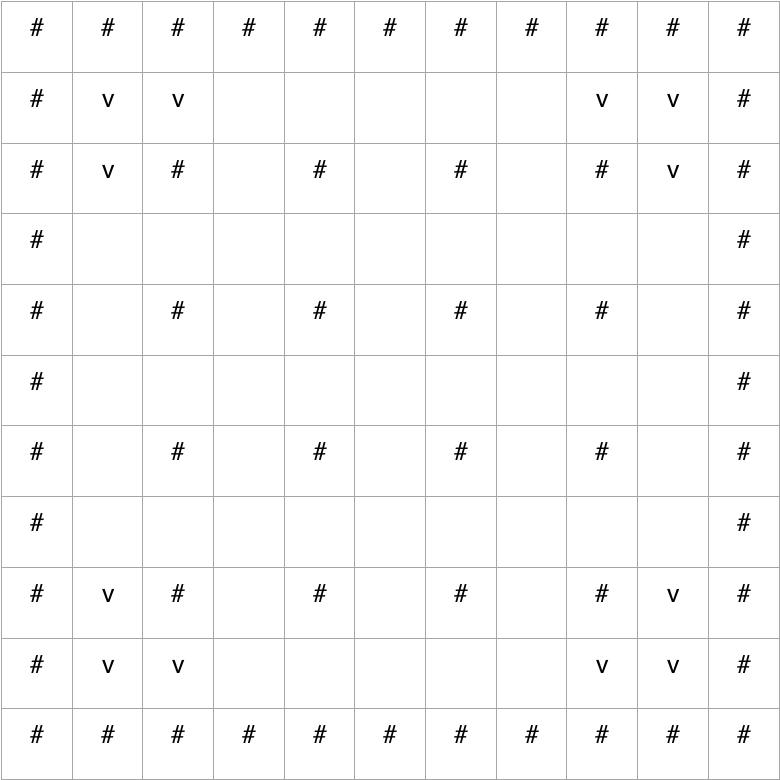
\includegraphics[scale = 0.5]{Mapa.png}
      \caption{Mapa de Bomberman (11x11)}
      \label{Rotulo}
\end{figure}

Decidimos desenvolver o mapa pensando que é composto por linhas .\par
As células vazias vão ser preenchidas com números pseudo-aleatórios que vão ser necessários para saber o que existe em cada célula. 

\newpage 

A tabela seguinte demonstra a distribuição dos número aleatórios e o que representam.

\begin{table}[H]
      \centering
      \caption{Distribuição dos número aleatórios}
      \label{my-label}
\begin{tabular}{|c|c|c|}
      \hline
\multicolumn{1}{|l|}{} & \multicolumn{1}{l|}{Número Aleatórios} & \multicolumn{1}{l|}{Representação} \\ \hline
Power-Up Bombs         & 0 - 1                                  & +                                  \\ \hline
Power-Up Flames        & 2 - 3                                  & !                                  \\ \hline
Tijolo                 & 4 - 39                                 & ?                                  \\ \hline
Célula Vazia           & 40 - 99                                & \multicolumn{1}{l|}{}              \\ \hline
\end{tabular}
\end{table}

Para este efeito, definimos duas funções, a função \emph{randomList} que nos devolve os números pseudo-aleatórios e a função \emph{tradutor} que vai atribuir a cada número aleatório a representação correspondente:

\vspace{0.5cm}

\begin{verbatim}
randomList :: Int -> Int -> [Int]
randomList size seed = take (numOpenSpace size) $ randomRs (0,99) (mkStdGen seed)

tradutor :: [Int] -> Bool -> String
tradutor [] _ = []
tradutor (h:t) n | h < 40 && n = '?' : tradutor t n
                 | h < 2 = '+' : tradutor t n
                 | h < 4 = '!' : tradutor t n
                 | otherwise = ' ' : tradutor t n 
\end{verbatim}

\vspace{0.5cm}

Após a conclusão da tarefa, obtemos o mapa do jogo como os power-ups e as posições dos mesmos abaixo da grelha do mapa.

\subsubsection{Exemplo da Tarefa 1}

O output da tarefa 1 é o mapa do jogo com a posição  dos power-ups abaixo da grelha do mapa. O mapa é dado através da função \emph{mapa}. No exemplo abaixo, dá-mos o exemplo do output da tarefa 1 no mapa de dimensão 13 e seed 9.

\begin{verbatim}
#############
#   ?  ?    #
# #?#?#?#?# #
#    ?      #
#?# # # #?# #
#?? ?????  ?#
# # # # # #?#
#? ?  ???   #
#?# #?# # # #
#  ?   ??? ?#
# # # # # # #
#   ?? ?    #
#############
+ 7 7
! 3 7
\end{verbatim}

\newpage

\subsection{Tarefa 2} O objetivo desta tarefa é a reação a comandos e a colocação de bombas. A lista de comandos sugerida pelos docentes foi a seguinte:

\vspace{0.5cm}

\begin{labeling}{Lista de Comandos}
      \item [U] Movimento para cima
      \item [D] Movimento para baixo 
      \item [L] Movimento para a esquerda
      \item [R] Movimento para a direita
      \item [B] Colocação de uma bomba
\end{labeling}

\vspace{0.5cm}

O jogador só se pode mover para células vazias, ou seja, caso uma célula esteja ocupada por um tijolo, o jogador terá que colocar uma bomba para destrui-lo e, caso a célula esteja ocupada por uma pedra, o mesmo não puderá avançar para essa posição. Para este efeito, definimos a função \emph{canMove} que testa se uma célula é vazia ou não.

\begin{verbatim}
canMove :: [String] -> (Int,Int) -> Bool
canMove [] _ = False
canMove l (x,y) | (l!!y)!!x == ' ' = True
                | otherwise = False
\end{verbatim}

Caso a célula esteja vazia, o jogador pode avançar para a posição pretendida e o estado do jogo é atualizado segundo a função \emph{drawAtPlayer}. Caso nessa célula exista um power-up, esse mesmo é adicionada à lista de power-ups do jogador (segundo a função auxiliar \emph{addPower})

\vspace{0.5cm}

\subsubsection{Exemplo da Tarefa 2}
O output desta tarefa é a implementação de bombas e a reação a comandos. Neste exemplo, os jogadores 0 e 1 encontram-se na posição 3 7 e 7 3, respetivamente e também foi colocada uma bomba de raio 1 e tempo de detonação 10 pelo jogador 0.

\begin{verbatim}
#############
#           #
# # # # # # #
#?   ??   ??#
#?# # # # # #
# ? ???   ??#
# # #?# #?# #
#         ? #
# # #?#?#?# #
# ?         #
# #?# #?#?# #
#  ??? ? ?  #
#############
+ 5 3
+ 2 5
! 3 8
! 3 11
* 0 3 7 1 10
0 3 7
1 7 3
\end{verbatim}

\subsection{Tarefa 3} A tarefa três é destinada à compressão e descompressão do jogo dado o estado atual do mesmo com objetivo de poupar espaço no disco do computador.\par Relativamente à compressão do jogo, primeiramente retiramos as pedras do contorno do mapa assim como as que se encontram em cada linha ou coluna, alternadamente, pois as pedras encontram-se sempre no mesma posição em cada mapa. De seguida, juntamos as repetições dos elementos do mapa e criámos um dicionário de compressão que vai ser apresentado de seguida.

\begin{table}[H]
      \centering
      \caption{Dicionário de compressão}
\begin{tabular}{|c|c|c|c|}
      \hline
\textbf{Letra} & \textbf{Significado}                                                   & \multicolumn{1}{l|}{\textbf{Letra}} & \multicolumn{1}{l|}{\textbf{Significado}}                  \\ \hline
\textbf{A}     & Espaço Vazio                                                           & \textbf{H}                          & \begin{tabular}[c]{@{}c@{}}Bomba\\ (Player 1)\end{tabular} \\ \hline
\textbf{B}     & Tijolo                                                                 & \textbf{I}                          & \begin{tabular}[c]{@{}c@{}}Bomba\\ (Player 2)\end{tabular} \\ \hline
\textbf{C}     & \begin{tabular}[c]{@{}c@{}}Power-Up Bombs\\ (Coberto)\end{tabular}     & \textbf{J}                          & \begin{tabular}[c]{@{}c@{}}Bomba\\ (Player 3)\end{tabular} \\ \hline
\textbf{D}     & \begin{tabular}[c]{@{}c@{}}Power-Up Bombs\\ (Descoberto)\end{tabular}  & \textbf{K}                          & Player 0                                                   \\ \hline
\textbf{E}     & \begin{tabular}[c]{@{}c@{}}Power-Up Flames\\ (Coberto)\end{tabular}    & \textbf{L}                          & Player 1                                                   \\ \hline
\textbf{F}     & \begin{tabular}[c]{@{}c@{}}Power-Up Flames\\ (Descoberto)\end{tabular} & \textbf{M}                          & Player 2                                                   \\ \hline
\textbf{G}     & \begin{tabular}[c]{@{}c@{}}Bomba\\ (Player 0)\end{tabular}             & \textbf{N}                          & Player 3                                                   \\ \hline
\end{tabular}
\end{table}

\vspace{0.5cm}

Observações relativamente à compressão:

\begin{itemize}
      \item As letras A,B,C,D,E e F movem a posição para a direita. O número anterior à letra corresponde ao número de vezes que se repete seguidamente.
      \item As quebras de linha são ignoradas.
      \item Nas letras G,H,I e J avança para a direita e, o número antes é o raio da bomba e o número posterior é o tempo de detonação da mesma. Se o tempo for 10, o número a seguir é 0.
      \item Nas letras K,L,M e N o número anterior à letra corresponde ao power-up bombs e o número posterior ao número de power-up flames que o jogador colectou. A seguir a este número é efectuado um espaço.
\end{itemize}

\vspace{0.5cm}

De seguida, tivemos que definir o processo inverso à compressão, a descompressão. Em primeiro lugar, a função \emph{decompressMap} calcula o tamanho do mapa, só depois é que aplica o processo de descompressão. 

\subsubsection{Exemplo da Tarefa 3}

O output da tarefa 3 dada pelas funções \emph{encode} e \emph{decode} é o jogo comprimido e descomprimido, respetivamente. A codificação abaixo é relativa à compressão de um mapa de dimensão 13 e de seed 9 onde a posição dos power-ups e dos jogadores também é comprimido.
\begin{verbatim}
"K3AB2AB3AL2A4B5AB6AB3ABA2BA5B2AB5A2BAD2ABCB3ABAB5AB3A3BAB9A2BAB4A"
\end{verbatim}

\newpage

A grelha abaixo é relativa à descompressão do código anunciado acima. O resultado é a grelha do mapa de dimensão 13 e seed 9.

\begin{verbatim}
#############
#   ?  ?    #
# #?#?#?#?# #
#    ?      #
#?# # # #?# #
#?? ?????  ?#
# # # # # #?#
#? ?  ???   #
#?# #?# # # #
#  ?   ??? ?#
# # # # # # #
#   ?? ?    #
#############
+ 7 7
! 3 7
0 1 1
1 11 1
\end{verbatim}

\subsection{Tarefa 4} O objetivo da tarefa quatro é passagem do tempo onde o efeito principal é a explosão de bombas e a morte de jogadores.\par O raio de uma bomba aumenta uma unidade com cada instante de tempo passado, e a bomba tem impacto nas quatro direções possíveis. A função \emph{radius} é o resultado após a explosão de uma bomba, onde o impacto dá-se nas quatro direções, cuja representação na função é dada pelas coordenadas \emph{right}, \emph{left}, \emph{down} e \emph{up}.

\begin{verbatim}
radius :: [String] -> (Int,Int) -> Int -> (Int,Int,Int,Int)
radius m (x,y) r = (rad right,rad left,rad down,rad up)
                  where rad d = radiusDir m (x,y) d 1 (r+1)
                        right = (1,0)
                        left = (-1,0)
                        down = (0,1)
                        up = (0,-1)
\end{verbatim}

\vspace{0.5cm}

O tempo de detonação de cada bomba é de 10 instantes de tempo, para esse efeito definimos as funções \emph{reduceTimeofBombs} e \emph{explodeBombs} que vão reduzir o tempo das bombas conforme a passagem do tempo e explodir a bomba, respetivamente.\par Cada jogo tem uma duração fixa e, para forçar os jogadores a fazer ações, o mapa (dimensão n) começa a fechar-se em efeito espiral quando o tempo é igual a $(n-2)^2$.\par  A espiral destroi bombas que ainda não detonaram, destroi power-ups e ainda pode matar jogadores se estes se encontrarem no caminho da mesma. Definimos, então, a função \emph{drawSpiral} que vai desenhar a espiral no mapa destruindo tudo por onde passa.

\vspace{0.5cm}

\subsubsection{Exemplo Tarefa 4}
Na tarefa 4 dá-se a passagem do tempo através da função \emph{avanca}. Dado um mapa e o tempo para o final do jogo, a função devolve o novo estado de jogo quando o tempo avança um instante. 
O exemplo seguinte é relativo à passsagem do tempo. Como input demos um mapa de dimensão 13 e seed 9 onde foi colocada uma bomba pelo jogador 0 na posição 3 1 com raio 2 e tempo de detonação 10. O mapa impresso terá uma modificação no tempo de detonação que passa de 10 para 9 devido à passagem de um instante de tempo.

\begin{verbatim}
#############
#   #  ?    #
# #?#?#?#?# #
#    ?      #
#?# # # #?# #
#?? ?????  ?#
# # # # # #?#
#? ?  ???   #
#?# #?# # # #
#  ?   ??? ?#
# # # # # # #
#   ?? ?    #
#############
+ 7 7
! 3 7
* 0 3 1 2 9
0 3 1
1 9 1
\end{verbatim}

\subsection{Tarefa 5}
\paragraph{} A tarefa cinco tem como objetivo a implementação do jogo completo usando a biblioteca \emph{Gloss}. A partir desta tarefa podemos ter uma noção gráfica do jogo.\par A ideia gráfica do nosso jogo consiste em Emoji's e numa ideia minimalista. Os emoji's são da autoria da EmojiOne, os quais são gratuitos e de livre uso, onde fizemos pequenas alterações para corresponder ao estilo do jogo.\par O mapa é centrado à esquerda com uma borda de 10px, o temporizador situa-se no canto superior direito e os players, que ainda estão em jogo, situam-se na parte direita da janela. Por fim, em baixo tem o botão "Pausar".\par Funcionalidades:

\begin{itemize}
      \item Pausar o jogo a qualquer momento.
      \item Mudar as dimensões do mapa
      \item Mudar o avatar do jogador
\end{itemize}

\subsubsection{Exemplos da Tarefa 5}

As imagens abaixo são prints do nosso trabalho desenvolvido em Gloss para a implementação dos gráficos do jogo.

\begin{figure}[H]
      \centering
      \caption{Exemplos da parte gráfica}
      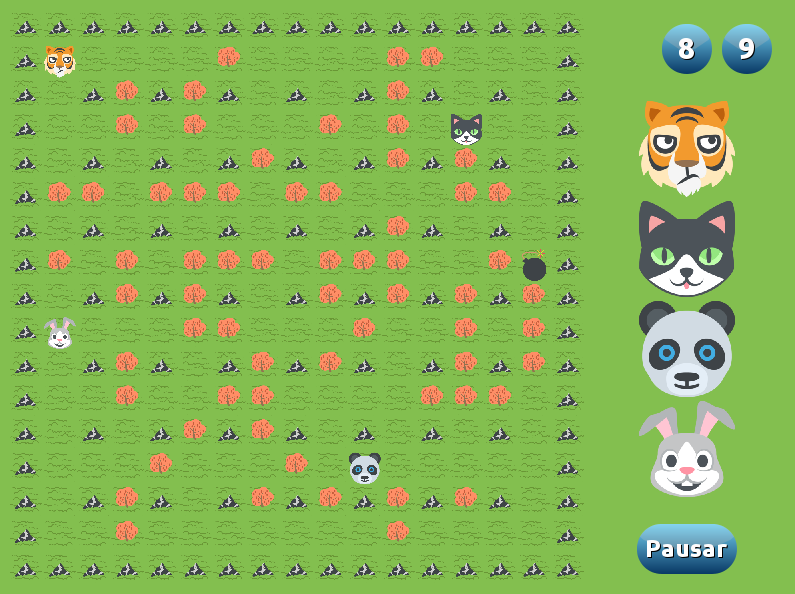
\includegraphics[scale=0.2]{jogo.png}
      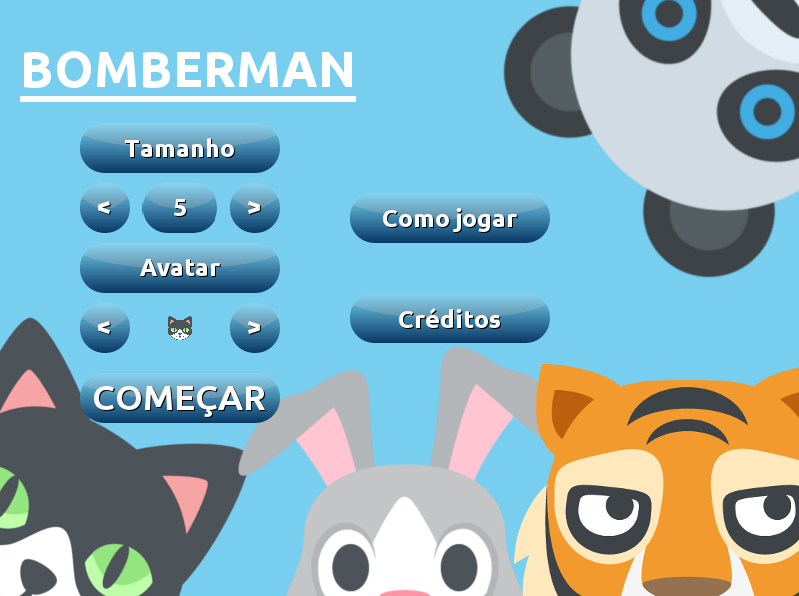
\includegraphics[scale=0.2]{jogo1.png}
\end{figure}

\vspace{0.5cm}

\subsection{Tarefa 6} Por fim, a tarefa seis tem como finalidade implementar estratégia de combate.\par O jogador tem quatro direções possíveis para praticar uma ação (cima, baixo, esquerda e direita). No entanto, algumas não são possíveis pois as células para qual o jogador se pretende mover podem conter pedras ou tijolos e também é possível que a célula pretendida seja considerada de risco pois pode conter uma bomba com tempo 0 ou pode fazer parte da espiral. A função \emph{canMove} vai verificar se o jogador pode praticar determinada ação.

\begin{verbatim}
canMove :: [String] -> Int -> Int -> Int -> [[Bool]]
canMove m t i z | i == z = map (map (<9) ) n
                | otherwise = canMove (avanca m (t-z)) t i (z+1)
                  where n = dangerMap m (t+z)
\end{verbatim}

No código da tarefa, representámos as ações de movimento como $(x,y+1)$,$(x,y-1)$,$(x+1,y)$ e $(x-1,y)$. O jogador vai verificar se é possível mover-se para a célula pretendida e, caso seja possível, vai adicionar à lista. Isto vai ser repetido 10 vezes e ao fim dessas repetições vai verificar o risco. O risco é um mapa que indica quantos instantes faltam para estar em situação muito perigosa, por exemplo, uma bomba de tempo 5 corresponde a 6 de risco, uma bomba de tempo 1 corresponde a 10 de risco e uma de tempo 10 corresponde a risco 1. A espiral também faz parte dos factores de risco, quanto mais perto da espiral maior é o risco, então a estratégia do jogador é manter-se afastado da espiral para não morrer.\par Após o jogador identificar todas as situações de risco, vai filtrar as situações que não são de risco e vai escolher a solução ótima. Caso não haja uma solução ótima, o jogador arranja uma situação de menos risco. Definimos a função \emph{goalMap} que arranja a melhor solução de ação para o jogador.

\begin{verbatim}
goalMap :: [String] -> [[Int]]
goalMap m = brickPriority n2 (listOfBricks m 0)
            where powers = listOfPowers m
                  p z (x,y) = (z!!y)!!x
                  n2 = drawAtPoints n powers 0
                  n = spiralIndex (1,1) (startSpiralIndex size size) ((size-2)^2) 'R'
                  size = length $ m!!0
\end{verbatim}

Os power-ups do mapa vão ser trocados por 0 e o jogador está definido a preferir esse local. Definimos também a redução dos números em torno dos tijolos para ele preferir os locais com mais tijolos e, à medida que o jogador se aproxima do centro esta definição terá cada vez menos importância.

\newpage

O output da tarefa será um dos seguintes movimentos:

\begin{labeling}{Lista de Comandos}
      \item [Just U] Movimento para cima
      \item [Just D] Movimento para baixo 
      \item [Just L] Movimento para a esquerda
      \item [Just R] Movimento para a direita
      \item [Just B] Colocação de uma bomba
      \item [Nothing] Não faz nada
\end{labeling}

\subsubsection{Exemplo da Tarefa 6}

O output da tarefa é movimento do jogador e vai ser dado pela função \emph{bot} que recebe como input o mapa, o jogador e o tempo que falta para o final da partida. Neste exemplo, o input é um mapa de dimensão 13 e seed 9 com os jogadores 0 e 1 nas posições 1 1 e 11 1, respetivamente. Decidimos que seria o jogador 0 a fazer um movimento no instante de tempo 120. O resultado foi o seguinte:

\begin{verbatim}
Just D
\end{verbatim}

\section{Conclusão}
O objetivo principal, que era a implementação do jogo Bomberman na linguagem funcional Haskell, foi alcançado. Conseguimos concluir todas as tarefas propostas pelos docentes da UC no tempo pretendido e conseguimos passar com êxito a todos os testes impostos no SVN.\par Este trabalho foi fundamental para uma melhor compreensão da linguagem funcional \emph{Haskell} e do seu funcionamento. Consideramos este trabalho de grande importância pois conseguimos desenvolver um raciocínio e método de trabalho que será fulcral para próximos trabalhos com outros tipos de linguagem. 

\end{document}
